\documentclass[twocolumn,english]{article}
\usepackage[latin9]{inputenc}
\usepackage[landscape]{geometry}
\geometry{verbose,tmargin=0.5in,bmargin=0.75in,lmargin=0.5in,rmargin=0.5in}
\setlength{\parskip}{0bp}
\setlength{\parindent}{0pt}
\usepackage{array}
\usepackage{float}
\usepackage{booktabs}
\usepackage{multirow}
\usepackage{amsmath}
\usepackage{graphicx}

\makeatletter

\providecommand{\tabularnewline}{\\}




\usepackage{array}
\usepackage{multirow}
\usepackage{amsbsy}




\providecommand{\tabularnewline}{\\}

\setlength{\columnsep}{0.25in}
\usepackage{xcolor}
\usepackage{textcomp}
\usepackage{listings}
\lstset{
  tabsize=2,
  basicstyle=\small\ttfamily,
}



\usepackage{babel}
\usepackage{listings}
\renewcommand{\lstlistingname}{Listing}

\AtBeginDocument{
  \def\labelitemii{\(\bullet\)}
}

\makeatother

\usepackage{babel}
\begin{document}

\title{Reference Sheet for C211 Operating Systems}

\date{Spring 2018}
\maketitle

\paragraph{Operating systems}

have to
\begin{itemize}
\item \emph{Manage resources}: processors, memory, IO, clocks, interrupt
controllers, storage.
\item \emph{Provide clean interfaces}: offer level of abstraction above
hardware.
\end{itemize}

\paragraph{Flavours}

E.g. server / supercomputer / smartphone / embedded operating systems.

\paragraph{Kernel}

Part of the OS that:
\begin{itemize}
\item Is always loaded in memory.
\item Executes in a privileged mode with access to all hardware.
\end{itemize}

\paragraph{Structure}
\begin{itemize}
\item \emph{Monolithic kernels}: single executable with its own address
space.
\begin{itemize}
\item $+$ Efficient calls within kernel.
\item $+$ Easier to write components due to shared memory.
\item $-$ Complex design with lots of interactions.
\item $-$ No protection between kernel components.
\end{itemize}
\item \emph{Microkernels}: minimal level kernel with functionality in user-level
servers.
\begin{itemize}
\item $+$ Kernel not complex so less error prone.
\item $+$ Servers have clean interfaces.
\item $+$ Servers can crash and restart without crashing kernel.
\item $-$ Overhead of IPC within kernel high.
\end{itemize}
\item \emph{Hybrid kernels}: combines features of each. Compromise between
clean design and performance overhead.
\end{itemize}

\section{Processes}

\paragraph{Process}

An instance of a program being executed.
\begin{itemize}
\item Provides illusion of concurrency.
\item Provides isolation between programs (each has its own address space).
\item Simplicity of programming (can assume complete control).
\item Allows better utilisation of resources.
\end{itemize}

\paragraph{Types of Concurrency}
\begin{itemize}
\item \emph{Pseudo concurrency}: single processor is switched between processes
by interleaving (e.g. by \emph{time-slicing}).
\item \emph{Real concurrency}: utilises multiple physical processors.
\end{itemize}

\paragraph{CPU Utilisation}

If we have $n$ processes, each with probability $p$ of waiting for
I/O at any time, expect CPU utilisation to be $1-p^{n}$.

\paragraph{Context Switch}

Processor switches from executing process $A$ to process $B$.
\begin{itemize}
\item OS may make scheduling decisions: may switch processes in response
to events/interrupts.
\item Adds non-determinism to execution (events occur in unpredictable order).
\item \emph{Expensive}: need to save/restore state, lost CPU caches (including
TLBs), ...
\end{itemize}

\paragraph{Process Control Block}

Each process has a \emph{process descriptor} or \emph{process control
block}, kept in the \emph{process table}.
\begin{itemize}
\item Process has its own virtual machine (CPU, address space, file descriptors,
...).
\item Need to store state:
\begin{itemize}
\item \emph{Registers}: PC, page table register, stack pointer, ...
\item \emph{Process management info}: ID, parent, group, priority, CPU used,
...
\item \emph{File management info}: root directory, working directory, open
FDs
\end{itemize}
\end{itemize}

\paragraph{Process Types}
\begin{itemize}
\item \emph{Foreground processes}: interact with users.
\item \emph{Background processes}: daemons.
\end{itemize}

\paragraph{Process Creation}

Can happen by system initialisation, user requests, system calls.

\paragraph{Process termination}
\begin{itemize}
\item \emph{Normal completion}: process completes execution of body.
\item \emph{System call}: call to \texttt{exit()}.
\item \emph{Abnormal exit}: run into error / unhandled exception.
\item \emph{Never}: e.g. (hopefully) web servers.
\end{itemize}

\paragraph{Process Hierarchies}

All processes form a process tree with \texttt{init} as the root (\emph{process
group}).

\paragraph{Creation and Termination}
\begin{itemize}
\item \texttt{fork()} creates a new child process with an exact copy of
parent. 
\begin{itemize}
\item In parent process, returns PID of child.
\item In child process, returns 0.
\end{itemize}
\item \texttt{execve(path, argv, envp)} executes a command.
\item \texttt{waitpid(pid, stat, option)} suspends execution of calling
process until \texttt{pid} terminates normally or a signal is received.
\begin{itemize}
\item \texttt{-1} waits for any child.
\item \texttt{0} waits for any child in the same process group as the caller.
\item \texttt{-gid} waits for any child with process group \texttt{gid}.
\end{itemize}
\item \texttt{exit(status)} terminates process (called implicitly).
\item \texttt{kill(pid, sig)} sends signal \texttt{sig} to \texttt{pid}.
\end{itemize}

\paragraph{Communicating between Processes}

Files, signals, pipes, message queues, sockets, shared memory, semaphores.

\paragraph{UNIX Signals}

Used to notify processes when an event occurs.
\begin{itemize}
\item User ID of the receiving process must match that of the sending process
or have appropriate privileges.
\item Kernel can send signal to any process.
\item \texttt{SIGFPE} division by 0, \texttt{SIFSEGV} segment violation,
\texttt{SIGPIPE} writes to closed pipe, \texttt{SIGINT} interrupted
process, ....
\item Process can ignore / handle signals (except \texttt{SIGKILL} and \texttt{SIGSTOP}).
\end{itemize}

\paragraph{UNIX Pipes}

Connects standard output of one process to standard input of another.
Allows \emph{one-way} communication.
\begin{itemize}
\item \texttt{pipe(fd{[}2{]})}: \texttt{fd{[}0{]}} is the read end and \texttt{fd{[}1{]}}
the write end of the pipe.
\item \emph{Named pipes} (FIFOs): persistent pipes that outlive process
which created them.
\begin{itemize}
\item Stored on the filesystem, but more efficient since it only exists
in memory.
\end{itemize}
\end{itemize}

\section{Threads}

Execution streams that share the same address space (each process
can contain one or more threads).

\begin{table}[H]
\centering{}%
\begin{tabular}{cc}
\toprule 
\textbf{Per process} & \textbf{Per thread}\tabularnewline
\midrule
Address space & PC\tabularnewline
Global variables & Registers\tabularnewline
Open files & Stack\tabularnewline
Child processes & \tabularnewline
Signals & \tabularnewline
\bottomrule
\end{tabular}
\end{table}

\paragraph{Uses}

Applications with multiple activities which:
\begin{enumerate}
\item Execute in parallel.
\item Access and process the same data.
\item May sometimes block.
\end{enumerate}
Processes are more heavyweight (difficult communication and expensive
creation / context switching / termination).

\paragraph{PThreads}
\begin{itemize}
\item \texttt{pthread\_create(thread, attr, start\_routine, arg)} creates
a new thread.
\item \texttt{pthread\_exit(value\_ptr)} terminates thread and makes \texttt{value\_ptr}
available to any join. Called implicitly when thread returns.
\begin{itemize}
\item If \texttt{main()} terminates, entire process is terminated, unless
\texttt{pthread\_exit()} is called (process executes until last thread
terminates or \texttt{exit()} is called).
\end{itemize}
\item \texttt{pthread\_yield()} releases CPU to let another thread run.
\item \texttt{pthread\_join(thread, value\_ptr)} blocks until thread terminates.
\end{itemize}

\paragraph{Implementation Options}
\begin{itemize}
\item \emph{User-level}: kernel is not aware of threads, each process manages
its own threads.
\begin{itemize}
\item Implemented by software library.
\item Process maintains \emph{thread table} for \emph{thread scheduling}.
\item $+$ Better performance (creation, termination, switching and joining
are fast since no kernel involvement required).
\item $+$ Each application can have its own scheduling algorithm.
\item $-$ Blocking system calls stops all threads in process. Non-blocking
I/O can be used (difficult to use).
\item $-$ During page fault, OS blocks whole process.
\end{itemize}
\item \emph{Kernel-level}: managed by the kernel.
\begin{itemize}
\item $+$ Blocking system calls / page faults are easily accommodated.
\item $-$ Thread creation and termination requires system calls so more
expensive (can use \emph{thread pools} to recycle threads).
\item $-$ Thread synchronisation requires blocking system calls so more
expensive.
\item $-$ Thread switching requires system calls so more expensive.
\item $-$ No application-specific schedulers.
\end{itemize}
\item \emph{Hybrid approach}: use kernel threads and multiple user-level
threads onto kernel-threads.
\end{itemize}

\section{Scheduling}

\begin{figure}[H]
\centering{}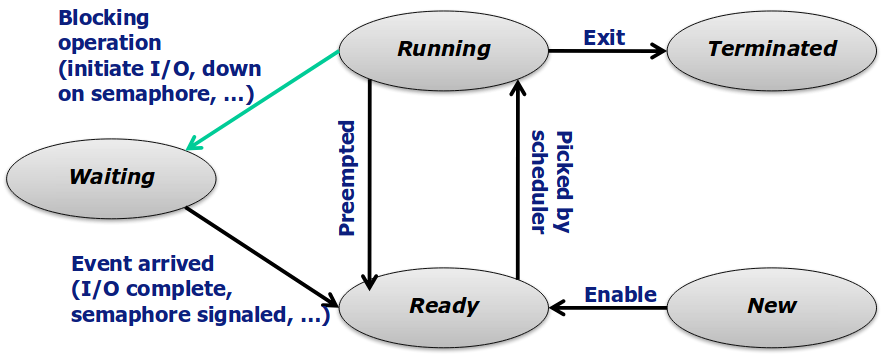
\includegraphics[width=0.75\linewidth]{img/process-states}
\end{figure}

\paragraph{Goals}
\begin{itemize}
\item Ensure fairness.
\item Avoid indefinite postponement.
\item Enforce policy (e.g. priorities).
\item Maximise resource utilisation (e.g. CPU, I/O devices).
\item Minimise overhead (from scheduling decisions and context switches).
\end{itemize}
\rule{0.25\columnwidth}{0.5pt}
\begin{itemize}
\item Batch systems: optimise for \emph{throughput} and \emph{turnaround
time}.
\item Interactive systems: optimise for \emph{response time}.
\item Real-time systems: meet deadlines.
\end{itemize}

\paragraph{Preemption}
\begin{itemize}
\item \emph{Non-preemptive}: let process run until it blocks or voluntarily
releases CPU.
\item \emph{Preemptive}: Let process run for a maximum amount of fixed time,
using clock interrupt.
\end{itemize}

\paragraph{Processes}
\begin{itemize}
\item \emph{CPU-bound}: spend most of their time using the CPU.
\item \emph{I/O-bound}: spend most of their time waiting for I/O and use
CPU only briefly.
\end{itemize}

\subsection{Scheduling Algorithms}

\paragraph{First-Come-First-Served}

Non-preemptive. Runnable process added to the end of ready queue.
\begin{itemize}
\item $+$ No indefinite postponement (all processes are eventually scheduled).
\item $+$ Really easy to implement.
\item $-$ Poor turnaround time if a long job is followed by many short
jobs.
\end{itemize}

\paragraph{Round Robin}

Run process until it blocks or time quantum exceeded.
\begin{itemize}
\item $+$ Fair: ready jobs get equal share of the CPU.
\item $+$ Good response time for small number of jobs.
\item $+$ Average turnaround time is low when run-times differ.
\item $+$ Average turnaround time is poor for similar run-times.
\end{itemize}
As quantum increases:
\begin{itemize}
\item $+$ Overhead decreases.
\item $-$ Response time worsens.
\end{itemize}
Quantum value should be:
\begin{itemize}
\item Much large than cost of a context switch,
\item But provide decent response time.
\end{itemize}

\paragraph{Shortest Job First}

Non-preemptive scheduling with run-times known in advance. Pick shortest
job first.
\begin{itemize}
\item $-$ Run-times not usually known in advance.
\begin{itemize}
\item Heuristics not always applicable.
\item User-supplied estimates encourage cheating (terminate processes if
they exceed estimate).
\end{itemize}
\end{itemize}

\paragraph{Shortest Remaining Time}

Preemptive version of shortest job first.

\paragraph{Fair-Share}

Round robin taking into account user that owns a process.

\paragraph{Lottery Scheduling}
\begin{itemize}
\item Jobs receive lottery tickets for various resources (e.g. CPU time).
\item At each scheduling decision, one ticket is chosen at random.
\item $+$ Highly responsive.
\item $+$ No starvation.
\item $+$ Jobs can exchange tickets (allows for priority donation, jobs
can cooperate).
\item $+$ Adding / removing jobs affect remaining jobs proportionally.
\item $-$ Unpredictable response time.
\end{itemize}

\subsection{Priority Scheduling}

Always run the job with the highest priority.
\begin{itemize}
\item Priorities could be externally defined or on some process-specific
metrics.
\item Priorities could be static or dynamic.
\end{itemize}

\paragraph{General-Purpose Scheduling}
\begin{itemize}
\item Favour short and I/O bound jobs.
\item Quickly determine the nature of the job and adapt to changes.
\end{itemize}

\paragraph{Multilevel Feedback Queues}

One queue for each priority level.
\begin{itemize}
\item Run job on highest non-empty priority queue.
\item Each queue can use a different scheduling algorithm (usually round
robin).
\item Need to worry about starvation of low-priority jobs:
\begin{itemize}
\item Recompute priorities periodically (e.g. based on how much CPU they've
used).
\item \emph{Ageing}: increase job's priority as it waits.
\end{itemize}
\item $-$ Not very flexible, priorities make no guarantees.
\item $-$ Does not react quickly to changes - often needs warm-up period.
\item $-$ Cheating is still a concern.
\item $-$ Cannot donate priority.
\end{itemize}

\section{Synchronisation}

\paragraph{Critical Section / Region}

Section of code in which processes access a shared resource.

\paragraph{Mutual Exclusion}

Ensures that if a process is executing its critical section, no other
process is executing it.
\begin{itemize}
\item Processes require \emph{permission} to enter critical sections - \emph{synchronisation
mechanism} required at entry and exit.
\end{itemize}
Requirements for mutual exclusion:
\begin{enumerate}
\item No two processes can be inside a critical section at the same time.
\item No process running outside the critical section can prevent other
processes from entering it.
\item No process requiring access to a critical section can be delayed forever.
\item No assumptions are made about relative speed of processes.
\end{enumerate}

\paragraph{Disabling Interrupts}
\begin{itemize}
\item Only works on single-processor systems.
\item Blocks I/O, preemptive scheduling, .... Only for short times used
by kernel code.
\end{itemize}

\paragraph{Strict Alternation}

Record whose `turn' it is.
\begin{itemize}
\item Violates requirement 2.
\item Busy waiting wastes CPU time (only OK when waiting for a short time).
\end{itemize}

\paragraph{Peterson's Solution}

Also record whether a thread is interested in entering critical region.

\paragraph{Atomic Operations}

A sequence of one or mare statements that is indivisible.
\begin{itemize}
\item \emph{TSL (Test and Set Lock) instruction}: atomically sets memory
location to 1 and returns old value.
\end{itemize}

\paragraph{Lock Variables}
\begin{enumerate}
\item \emph{Spin lock}: lock using busy waiting.
\begin{itemize}
\item Wastes CPU so only should be used when wait is short.
\item May run into \emph{priority inversion problem}.
\end{itemize}
\item \emph{Read/Write lock}: in write mode, thread has exclusive access;
in read mode, multiple threads can access.
\end{enumerate}

\paragraph{Lock Metrics}
\begin{itemize}
\item \emph{Lock granularity}: the amount of data a lock is protecting.
\item \emph{Lock overhead}: measure of cost of using locks (memory space,
initialisation, time required to acquire and release).
\item \emph{Lock contention}: measure of number of processes waiting for
lock.
\end{itemize}
To minimise contention / maximise concurrency:
\begin{enumerate}
\item Choose finer lock granularity.
\item Make critical sections small.
\item Use a different lock (e.g. read/write).
\end{enumerate}

\paragraph{Race Condition}

Occurs when multiple threads or processes read and write shared data
and the final result depends on the relative timing of their execution.

\paragraph{Memory Models}

Assume \emph{sequential consistency}: operations of each thread are
in program order.

\paragraph{Happens-Before Relationship}

Partial order between events in a trace. E.g. for $a,b$ with $a$
occurring before $b$ in the trace:
\begin{itemize}
\item If $a,b$ are in the same thread, then $a\rightarrow b$.
\item if $a$ is \texttt{unlock(L)} and $b$ is \texttt{lock(L)}, then $a\rightarrow b$.
\item Irreflexive, antisymmetric and transitive.
\end{itemize}
So a data race occurs between $a,b$ in trace iff:
\begin{enumerate}
\item They access the same memory location.
\item At least one is a write.
\item They are unordered according to happens-before.
\end{enumerate}

\paragraph{Semaphores}

Process cooperate by means of signals (process will continue if it
receives a signal). Special variable with atomic operations:
\begin{enumerate}
\item \texttt{down(s)}: receive a signal via a semaphore \texttt{s}.
\item \texttt{up(s)}: transmit a signal via semaphore \texttt{s}.
\item \texttt{init(s, i)}: initialise semaphore \texttt{s} with value \texttt{i}.
\end{enumerate}
\begin{itemize}
\item Implemented using a \texttt{counter} and a \texttt{queue} of waiting
processes.
\item Initial \texttt{counter} indicates how many process can access shared
data at same time.
\item Useful for mutual exclusion, ordering events.
\end{itemize}

\paragraph{Producer/Consumer}

Easily implemented with three semaphores:
\begin{itemize}
\item Producer can only deposit in buffer if there is space and mutex is
ensured.
\item Consumer can only fetch from buffer if it is non-empty and mutex is
ensured.
\item Buffer can hold $0$ to $N$ items.
\end{itemize}

\paragraph{Monitors}

Made up of:
\begin{itemize}
\item \emph{Shared data}.
\item \emph{Entry procedures} (called from outside monitor) and \emph{internal
procedures}.
\item An implicit monitor \emph{lock}.
\item \emph{Condition variables} associated with high-level conditions:
\begin{itemize}
\item \texttt{wait(c)}: releases monitor lock and waits for \texttt{c} to
be signalled.
\item \texttt{signal(c)}: wakes up one process waiting for \texttt{c}.
\item \texttt{broadcast(c)}: wakes up all processes waiting for \texttt{c}.
\end{itemize}
\end{itemize}
Different semantics possible:
\begin{itemize}
\item \emph{Hoare}: process waiting for signal is immediately scheduled.
\begin{itemize}
\item $+$ Easy to reason about.
\item $-$ \emph{Inefficient}: forces a context switch, places extra constraints
on scheduler.
\end{itemize}
\item \emph{Lampson}: sending signal and waking up from a wait not atomic.
\begin{itemize}
\item $-$ More difficult to understand (\texttt{wait()} usually needs to
be called in a \texttt{while} loop).
\item $+$ More efficient.
\item $+$ \emph{More robust}: if condition is wrong, it gets discarded
when rechecked.
\end{itemize}
\end{itemize}

\section{Deadlocks}

Set of processes is \emph{deadlocked} if each process is waiting for
an event that only another process can cause.

\paragraph{Requirements}
\begin{itemize}
\item \emph{Mutual exclusion}: each resource is either available or assigned
to exactly one process.
\item \emph{Hold and wait}: process can request resources while it holds
other resources earlier.
\item \emph{No preemption}: resources given to a process earlier cannot
be forcibly revoked.
\item \emph{Circular wait}: two or more processes in a circular chain, each
waiting for a resource held by the next process.
\end{itemize}

\paragraph{Resource Allocation Graph}

Directed graph in which:
\begin{itemize}
\item Arc from resource to process = process currently owns resource.
\item Arc from process to resource = process blocked waiting for resource.
\item Cycle = deadlock.
\end{itemize}

\paragraph{Handling Deadlocks}
\begin{enumerate}
\item \emph{Ignore it}: fine if contention for resources is low.
\item \emph{Detection and recovery}.
\begin{enumerate}
\item \emph{Detection}: dynamically build resource ownership graph and look
for cycles.
\item \emph{Recovery}:
\begin{enumerate}
\item \emph{Preemption}: temporarily take resource from owner and give to
another (hard).
\item \emph{Rollback}: checkpoint states, and rollback on deadlock.
\item \emph{Killing processes}: select a random process and cycle and kill
it.
\end{enumerate}
\end{enumerate}
\item \emph{Dynamic avoidance}: dynamically consider request and whether
it is safe to grant it.
\begin{enumerate}
\item \emph{Banker's algorithm}: a state is \emph{safe} iff there exists
a sequence of allocations that guarantees \emph{all} customers can
be satisfied.
\end{enumerate}
\item \emph{Prevention}: ensure at least one of the four deadlock conditions
never holds.
\begin{enumerate}
\item \emph{Mutual exclusion}: try to share the resource.
\item \emph{Hold and wait}: require all processes to request resources before
start (need to know what you need in advance).
\item \emph{No preemption}: force process to give up resource (often hard).
\item \emph{Avoid circular wait}: force single resource per process OR enforce
global order of resources.
\end{enumerate}
\end{enumerate}

\paragraph{Communication Deadlock}

Use reliable communication protocol based on timeouts.

\paragraph{Livelock}

Processes/threads not blocked but not making progress. E.g.
\begin{itemize}
\item Entering critical section fails and cause another attempt.
\item System receiving and processing messages, where processing thread
has lower priority and never gets a chance to run (\emph{receive livelock}).
\end{itemize}

\paragraph{Starvation}

Want all processes to eventually get resource they need.

\section{Memory Management}

\paragraph{Logical and Physical Addresses}
\begin{itemize}
\item \emph{Logical address}: generated by CPU, address seen by process.
\item \emph{Physical address}: address seen by memory unit.
\item \emph{Same} in compile-time and load-time address-binding schemes.
\item \emph{Different} in execution-time address-binding scheme.
\item \emph{Memory management unit} is a hardware device for mapping from
logical to physical addresses.
\end{itemize}

\paragraph{Contiguous Memory Allocation}

Separate main memory into two partitions
\begin{itemize}
\item \emph{Kernel}: held in low memory with interrupt vector.
\item \emph{User}: held in high memory.
\end{itemize}
\emph{Contiguous allocation} with \emph{relocation registers}:
\begin{itemize}
\item \emph{Base register} contains value of smallest physical address.
\item \emph{Limit register} contains range of logical addresses.
\item MMU maps logical addresses.
\item Check that base $\leq$ address $<$ base + limit.
\end{itemize}

\paragraph{Multiple-Partition Allocation}
\begin{itemize}
\item \emph{Hole}: block of available memory.
\item OS maintains info about allocated and free partitions.
\item New processes get allocated memory from a large enough whole.
\end{itemize}
Dynamic storage allocation:
\begin{itemize}
\item \emph{First-fit}: allocate first whole that is big enough.
\item \emph{Best-fit}: allocate smallest hole that is big enough (must search
entire list, unless it is ordered).
\end{itemize}
\emph{Fragmentation}:
\begin{itemize}
\item \emph{External}: total memory exists to satisfy request but is not
contiguous.
\item \emph{Internal}: allocated memory larger than request memory.
\end{itemize}
Can be reduced by \emph{compaction}: move contents of memory into
one large block (leads to I/O bottlenecks).

\paragraph{Swap}

Only running processes need to be kept in memory. Temporarily swap
other processes out of memory.
\begin{itemize}
\item Swap space can be file or a disk partition.
\item Transfer time is a major part of swap time.
\end{itemize}

\subsection{Virtual Memory with Paging}

Separation of user logical memory from physical memory:
\begin{itemize}
\item Only part of process needs to be in memory for execution.
\item Logical address space can be much larger than physical.
\item Address spaces can be shared by several processes.
\item Allows for more efficient process creation.
\end{itemize}

\paragraph{Paging}

Logical address space of process can be noncontiguous.
\begin{itemize}
\item \emph{Frames}: fixed size block of physical memory (OS keeps track
of free frames).
\item Pages: block of same size of logical memory.
\end{itemize}
Running a program:
\begin{enumerate}
\item Find free frames and load program.
\item Set up page table to translate logical to physical addresses.
\end{enumerate}

\paragraph{Address Translation}

Address generated by CPU is separated into:
\begin{itemize}
\item Page number $p$ (index into page table, which has base address of
pages in physical memory).
\item Page offset $d$ (defines physical memory address sent to memory unit).
\item For logical address space $2^{m}$ bytes and page size $2^{n}$ bytes:
\begin{itemize}
\item Page number is first $m-n$ bits.
\item Page offset is last $n$ bits.
\end{itemize}
\end{itemize}
\begin{figure}[H]
\centering{}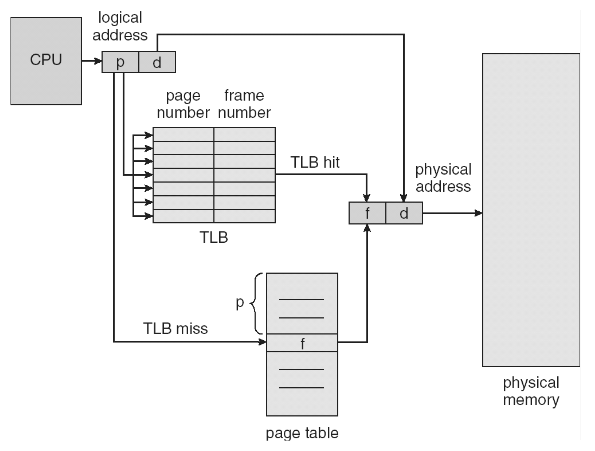
\includegraphics[width=0.75\linewidth]{img/address-translation}
\end{figure}

\paragraph{Memory Protection}

Associate protection bits with pages.
\begin{itemize}
\item Valid bit indicates legal page (page is in process's logical address
space).
\item Invalid bit indicates missing page (page fault - need to load page
/ may be incorrect address).
\end{itemize}
\begin{figure}[H]
\centering{}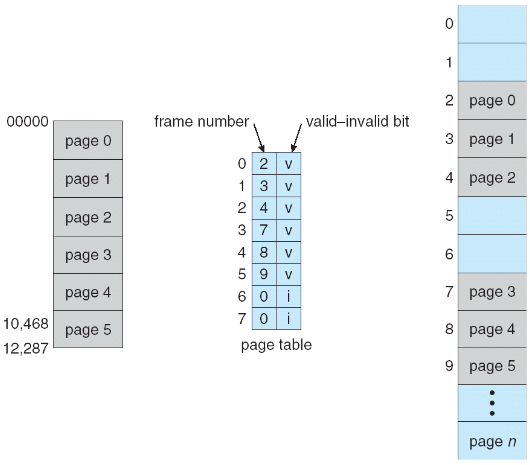
\includegraphics[width=0.6\linewidth]{img/page-table}
\end{figure}

\paragraph{Page Table Implementation}

Kept in main memory.
\begin{itemize}
\item \emph{Page-table base register} points to page table.
\item \emph{Page-table size register} indicates size.
\end{itemize}

\paragraph{Translation Look-aside Buffers}

Use a hardware cache as associative memory (from page to frame).
\begin{itemize}
\item Some TLBs store address-space IDs which uniquely identify processes.
\item TLBs usually need to flushed after context switch.
\end{itemize}

\paragraph{Effective Access Time}

Given associative lookup = $\epsilon$, memory cycle time = $1\mu$sec,
hit ratio = $\alpha$.
\[
\text{EAT}=(\epsilon+1)\alpha+\left(\epsilon+2\right)\left(1-\alpha\right)=2+\epsilon-\alpha
\]

\paragraph{Shared Memory}

Map pages from two processes to the same physical frame.
\begin{itemize}
\item \emph{Efficient}: no need for kernel involvement.
\item \emph{Flexible}: bidirectional by default.
\item Less useful for unidirectional communication (lack of \emph{synchronisation}).
\end{itemize}

\paragraph{Hierarchical Page Table}

Break up logical address space into multiple page tables. E.g. two-level
paging:
\begin{itemize}
\item More space efficient by allowing gaps in virtual address space.
\item Addresses now require two page numbers, followed by offset.
\item TLB misses now require two lookups!
\end{itemize}

\paragraph{Hashed Page Table}

Hash virtual page number into page table.
\begin{itemize}
\item Page table now contains linked list of elements hashing to same location.
\end{itemize}

\paragraph{Inverted Page Table}

Store an entry per frame instead of per page.
\begin{itemize}
\item Now need to search page table.
\end{itemize}

\subsection{Demand Paging}
\begin{itemize}
\item Bring page into memory only when needed:
\begin{itemize}
\item $+$ Lowers I/O load.
\item $+$ Less memory needed.
\item $+$ Faster response time.
\end{itemize}
\item Use invalid bits to cause a page fault.
\end{itemize}

\paragraph{Page Fault}

Operating system works out whether reference is valid or not. If valid
but just not in memory:
\begin{enumerate}
\item Get an empty frame.
\item Swap page into frame.
\item Set the valid bit in the page table to 1.
\item Restart last instruction.
\end{enumerate}

\paragraph{Effective Access Time}

For page fault rate $p$:
\begin{multline*}
\text{EAT}=\left(1-p\right)\times\text{memory access}+p(\text{page fault overhead}+\text{[swap page out]}\\
+\text{swap page in}+\text{restart overhead})
\end{multline*}

\paragraph{Optimisations}
\begin{itemize}
\item \emph{Copy-on-write}: parent process shares frames with child (as
read-only), and copy only happens on page fault.
\item \emph{Memory mapped files}: map file into virtual address space using
paging.
\end{itemize}

\paragraph{Page Replacement}

When there are no free frames, we need to find an unused page in memory
to swap out.
\begin{enumerate}
\item \emph{Minimise page faults}: avoid bringing same page into memory
several times.
\item \emph{Prevent over-allocation}: implement page replacement.
\item \emph{User dirty bit to reduce overhead}: only write modified pages
back to disk.
\end{enumerate}

\paragraph{FIFO Algorithm}

Replace the oldest page.
\begin{itemize}
\item $-$ May replace heavily used page.
\item Belady's anomaly: more frames $\rightarrow$ more page faults.
\end{itemize}

\paragraph{Optimal Algorithm}

Replace page that won't be used for longest period of time.
\begin{itemize}
\item $-$ Can't do this in practice!
\end{itemize}

\paragraph{Least Recently Used Algorithm}

When a page referenced, copy clock into \texttt{counter}. Choose lowest
\texttt{counter}.
\begin{itemize}
\item $-$ \emph{Expensive}: can't be done easily in hardware.
\item Approximation: use a \emph{reference bit}, which are periodically
restored. Choose page with ref bit 0.
\end{itemize}

\paragraph{Second Chance}

Use a reference bit, and walk through in clock order.

\paragraph{Counting Algorithms}
\begin{itemize}
\item \emph{Least frequently used}: replace page with smallest count.
\begin{itemize}
\item $-$ May replace page just brought into memory.
\item $-$ Never forgets heavy page usage.
\end{itemize}
\item \emph{Most frequently used}: replace page with largest count (page
with smallest count probably just brought in).
\end{itemize}

\paragraph{Locality of Reference}
\begin{itemize}
\item Want to maintain a program's favoured subset of pages.
\item \emph{Locality of reference}: programs usually request same pages
in space and time.
\item \emph{Thrashing}: excessive paging causes low processor utilisation
as program repeatedly requests pages.
\end{itemize}

\paragraph{Working Set Model}

\emph{Working set} $W\left(t,w\right)$ is set of pages referenced
during interval $t-w$ to $t$.
\begin{itemize}
\item Observe page fault frequency: if many faults, allocate more frames.
\end{itemize}

\paragraph{WS Clock Algorithm}

Require both reference bit unset \emph{and} page not in working set.

\paragraph{Global vs Local Page Replacement}
\begin{itemize}
\item \emph{Local}: each process gets fixed allocation of physical memory.
Need to pick up changes in WS size.
\item \emph{Global}: dynamically share memory between runnable processes.
Consider \emph{page fault frequency} to tune allocation.
\end{itemize}

\section{Device Management}

\paragraph{Objectives}
\begin{enumerate}
\item Allow fair access to shared devices.
\item Exploit parallelism of I/O devices.
\item Provide uniform simple view of I/O (hide complexity, make naming /
error handling uniform).
\end{enumerate}

\paragraph{Device Variations}

\emph{Block} devices use a buffer cache. \emph{Character} devices
don't.

\paragraph{I/O Layers}
\begin{enumerate}
\item \emph{User level I/O software}: provides user interface:
\begin{itemize}
\item Operations \texttt{open}, \texttt{close}, \texttt{read}, \texttt{write},
\texttt{seek}.
\item UNIX: access virtual devices as files.
\end{itemize}
\item \emph{Device-independent operating system software}: provides device
independence (from type and instance).
\begin{itemize}
\item Maps logical to physical devices.
\item Requests validation against device characteristics.
\item Allocates dedicated devices.
\item Validates user access.
\item Implements buffering.
\item Reports errors.
\end{itemize}
\item \emph{Device drivers/handlers}: handle one device type.
\begin{itemize}
\item Implements read/write.
\item Accesses device registers.
\item Initiates operations.
\item Schedules requests.
\item Handles errors.
\end{itemize}
\item \emph{Interrupt handlers}: process each interrupt.
\begin{itemize}
\item Block devices: on transfer completion, signals device handler.
\item Character devices: when character transferred, process next character.
\end{itemize}
\end{enumerate}

\paragraph{Dedicated Devices}

Either \emph{fail} if already opened or \emph{queue} open requests.

\paragraph{Shared Devices}

E.g. OS provides file system for disks.

\paragraph{Spooling}

Avoid blocking user access to allocated, non-sharable devices. E.g.
for printers:
\begin{enumerate}
\item Save printer output to disk file.
\item Print file later by \emph{spooler daemon} (only spooler daemon permitted
access to printer).
\end{enumerate}

\paragraph{Buffered I/O}
\begin{itemize}
\item \emph{Output}: transferred to OS output buffer, process only suspends
when buffer is full.
\item \emph{Input}: OS reads ahead, process blocks only when buffer is empty.
\end{itemize}

\paragraph{Unbuffered I/O}
\begin{itemize}
\item Data transferred directly from user space to/from device (each read/write
causes physical I/O).
\item High process switching overhead.
\end{itemize}

\paragraph{Memory-Mapped I/O}

Devices addressed as memory locations.

\paragraph{Ways to do I/O}
\begin{enumerate}
\item \emph{Programmed I/O}: continually poll until ready.
\item \emph{Interrupt-driven I/O}: initiate transfer, interrupt when complete.
\item \emph{I/O using DMA}: DMA controller transfers and interrupts when
complete.
\end{enumerate}

\paragraph{Blocking I/O}
\begin{itemize}
\item I/O call returns when operation completed.
\item Process suspended during I/O.
\end{itemize}

\paragraph{Non-blocking I/O}
\begin{itemize}
\item I/O call returns as much as available.
\item Provides application-level polling for I/O.
\end{itemize}

\paragraph{Asynchronous I/O}
\begin{itemize}
\item Process executes in parallel with I/O operation.
\item I/O systems notify process upon completion (e.g. by callback function).
\item Very efficient, but difficult to use and less secure.
\end{itemize}

\section{Disk Management}

\begin{figure}[H]
\centering{}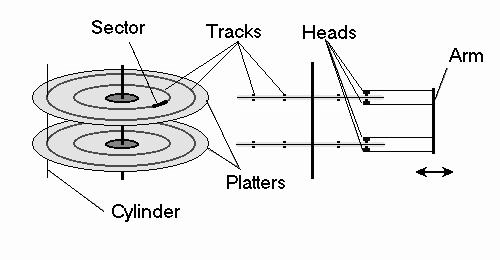
\includegraphics[width=0.4\linewidth]{img/disk}
\end{figure}

\paragraph{Sector Layout}

Surface divided into 20 or more zones.
\begin{itemize}
\item Outer zones have more sectors per track (so sectors have same physical
length).
\item Zones hidden using virtual geometry.
\end{itemize}

\paragraph{Disk Addressing}

Physical hardware addresses have form (cylinder, surface, sector).
Use \emph{logical sector addressing} / \emph{logical block addressing}:
sectors numbered consecutively.

\paragraph{Disk Formatting}
\begin{itemize}
\item \emph{Low level format}: adds structure to each sector (e.g. preamble,
error correcting code).
\item \emph{High level format}: adds filesystem structure, partitions, ....
\end{itemize}

\paragraph{Disk Delay}

Seek time + latency time (rotational delay) + transfer rate. Where
$b$ is bytes transferred, $N$ is bytes per track, and $r$ is rotation
speed in revolutions per second.
\[
t_{access}=t_{seek}+\frac{1}{2r}+\frac{b}{rN}
\]

\paragraph{Solid State Drives}
\begin{itemize}
\item More bandwidth.
\item Smaller latencies.
\item Much higher cost per unit storage.
\end{itemize}

\subsection{Disk Scheduling}

\paragraph{First Come First Serve}

No ordering of requests $\rightarrow$ random seek patterns.
\begin{itemize}
\item $+$ OK for lightly loaded disks.
\item $+$ Fair scheduling.
\item $-$ Poor performance for heavy loads.
\end{itemize}

\paragraph{Shortest Seek Time First}

Order requests according to shortest seek distance from current head
position.
\begin{itemize}
\item $-$ Discriminates against innermost / outermost tracks (unpredictable
and unfair).
\end{itemize}

\paragraph{SCAN / Elevator Scheduling}

Choose requests which result in shortest seek time in preferred direction.
(Only change direction when no further requests in preferred direction).
\begin{itemize}
\item $-$ Long delays for requests at extreme locations.
\end{itemize}

\paragraph{C-SCAN Scheduling}

Services requests in one direction only. (Jump to outermost request
after innermost).
\begin{itemize}
\item $+$ Lower variance of requests on extreme tracks.
\item $-$ May delay requests indefinitely (but unlikely).
\end{itemize}

\paragraph{N-Step SCAN}

Services only requests when sweep began. (Requests arriving during
sweep serviced during return sweep).
\begin{itemize}
\item $+$ Doesn't delay requests indefinitely.
\end{itemize}

\subsection{RAID}

Redundant Array of Inexpensive Disks.
\begin{itemize}
\item Use array of physical drives appearing as single virtual drive.
\item Stores data distributed over array of physical disks to allow parallel
operating (\emph{striping}).
\item Use redundant disk capacity to respond to disk failure.
\end{itemize}
\begin{figure}[H]
\centering{}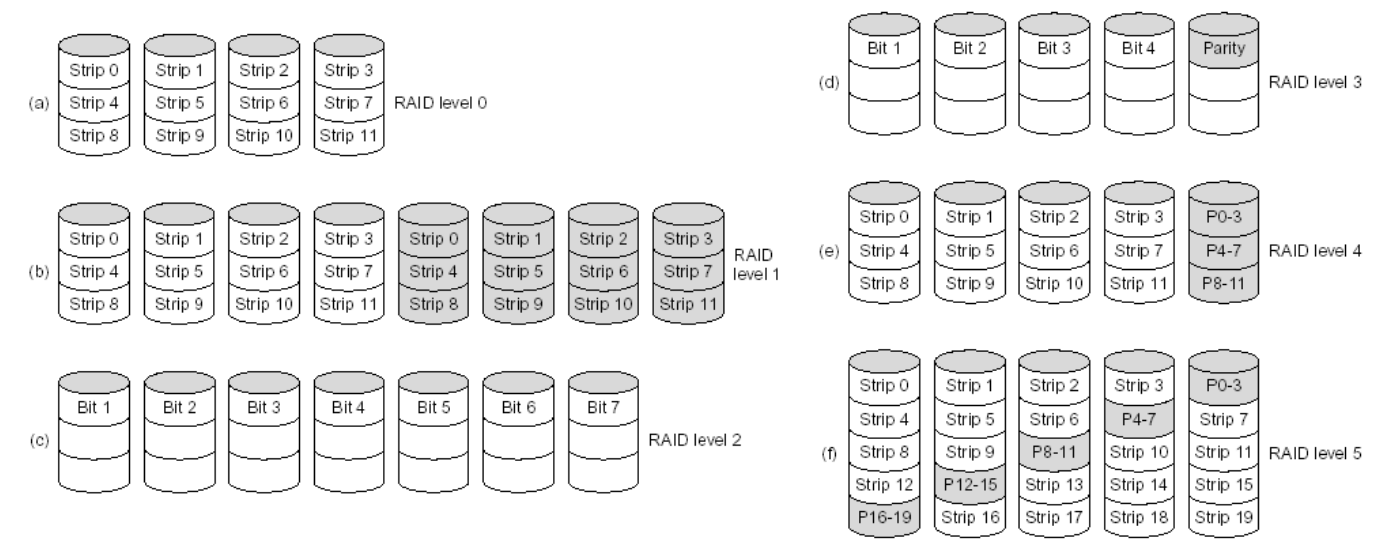
\includegraphics[width=0.95\linewidth]{img/raid}
\end{figure}

\paragraph{RAID 0 (Striping)}
\begin{itemize}
\item $+$ Disk can seek / transfer concurrently.
\item $-$ No redundancy $\rightarrow$ no fault tolerance.
\end{itemize}

\paragraph{RAID 1 (Mirroring)}
\begin{itemize}
\item $+$ Reads can be serviced by either disk (fast).
\item $+$ Failure recovery easy.
\item $-$ Writes must update both disks in parallel.
\item $-$ High storage overhead.
\end{itemize}

\paragraph{RAID 2 (Bit-Level Hamming)}
\begin{itemize}
\item $+$ Corrects single-bit errors (and detect double-bit errors).
\item $+$ Very high throughput (read all disks in parallel).
\item $-$ All disks participate in I/O requests (no concurrency).
\item $-$ Read-modify-write cycle to keep ECC bits correct.
\end{itemize}

\paragraph{RAID 3 (Byte-Level XOR)}
\begin{itemize}
\item $+$ Lower storage overhead than RAID 2.
\item $-$ Only one I/O request can take place at a time.
\end{itemize}

\paragraph{RAID 4 (Block-Level XOR)}
\begin{itemize}
\item $+$ Can service multiple reads concurrently.
\item $-$ Parity disk becomes bottleneck.
\end{itemize}

\paragraph{RAID 5 (Block-Level Distributed XOR)}
\begin{itemize}
\item $+$ Good efficiency/redundancy trade-off (some potential for write
concurrency).
\item $-$ Reconstruction of failed disk non-trivial.
\end{itemize}
\begin{table}[H]
\centering{}%
\begin{tabular}{>{\raggedright}p{1.5cm}c>{\centering}p{2.5cm}>{\centering}p{2.5cm}>{\centering}p{2.5cm}}
\toprule 
\textbf{\footnotesize{}Category} & \textbf{\footnotesize{}Level} & \textbf{\footnotesize{}Description} & \textbf{\footnotesize{}I/O Data Transfer} & \textbf{\footnotesize{}I/O Request Rate}\tabularnewline
 &  &  & {\footnotesize{}(Read / Write)} & {\footnotesize{}(Read / Write)}\tabularnewline
\midrule 
{\footnotesize{}Striping} & {\footnotesize{}0} & {\footnotesize{}Non-redundant} & {\footnotesize{}$+$ / $+$} & {\footnotesize{}$+$ / $+$}\tabularnewline
\midrule 
{\footnotesize{}Mirroring} & {\footnotesize{}1} & {\footnotesize{}Mirrored} & {\footnotesize{}$+$ / $0$} & {\footnotesize{}$+$ / $0$}\tabularnewline
\midrule 
\multirow{2}{1.5cm}{{\footnotesize{}Parallel Access}} & {\footnotesize{}2} & {\footnotesize{}Redundant via Hamming code} & {\footnotesize{}++ / ++} & {\footnotesize{}$0$ / $0$}\tabularnewline
 & {\footnotesize{}3} & {\footnotesize{}Bit interleaved parity} & {\footnotesize{}++ / ++} & {\footnotesize{}$0$ / $0$}\tabularnewline
\midrule 
\multirow{2}{1.5cm}{{\footnotesize{}Independent Access}} & {\footnotesize{}4} & {\footnotesize{}Block interleaved parity} & {\footnotesize{}$+$ / $-$} & {\footnotesize{}$+$ / $-$}\tabularnewline
 & {\footnotesize{}5} & {\footnotesize{}Block interleaved distributed parity} & {\footnotesize{}$+$ / $-$} & {\footnotesize{}$+$ / $-$ or $0$}\tabularnewline
\bottomrule
\end{tabular}
\end{table}

\subsection{Disk Caching}

Use main memory to improve disk access.
\begin{itemize}
\item \emph{Buffer} in memory for disk sectors, managed in terms of blocks
(multiple sectors for efficiency).
\item Buffer uses finite space (so needs replacement policy).
\end{itemize}

\paragraph{Least Recently Used}

Replace block that was in cache the longest with no references.
\begin{itemize}
\item Cache consists of \emph{stack} of blocks, implemented with \emph{pointers}.
\item $-$ Doesn't keep track of block popularity.
\end{itemize}

\paragraph{Least Frequency Used}

Replace block that has experience fewest references.
\begin{itemize}
\item Counter associated with each block (incremented with each access).
\item $-$ Some blocks may be referenced many times in short period.
\end{itemize}

\paragraph{Frequency-Based Replacement}

Divides LRU stack into a new and old section. Evict lowest count from
old block.
\begin{itemize}
\item Reference blocks move to the top of stack.
\item Reference count only updated if not in new section.
\item $-$ Blocks may age out too quickly: add a middle section from which
blocks can't be evicted.
\end{itemize}

\section{File Systems}

\section{Security}
\end{document}
